\documentclass[a4paper,12pt]{article} % This defines the style of your paper
\usepackage[brazilian]{babel} 
\usepackage[top = 2.5cm, bottom = 2.5cm, left = 2.5cm, right = 2.5cm]{geometry} 

\usepackage[T1]{fontenc}
\usepackage[utf8]{inputenc}

\usepackage{multirow} 
\usepackage{booktabs}
\usepackage{amsmath}
\usepackage{graphicx} 
\usepackage{amsmath}
\usepackage{setspace}
\setlength{\parindent}{0in}

% Package to place figures where you want them.
\usepackage{float}

% The fancyhdr package let's us create nice headers.
\usepackage{fancyhdr}

% To make our document nice we want a header and number the pages in the footer.

\pagestyle{fancy} % With this command we can customize the header style.

\fancyhf{} % This makes sure we do not have other information in our header or footer.

\lhead{\footnotesize Trabalho1 - LaTex}% \lhead puts text in the top left corner. \footnotesize sets our font to a smaller size.

%\rhead works just like \lhead (you can also use \chead)
\rhead{\footnotesize Daniel Magalhães Nunes, Francilene da Silva Sales} %<---- Fill in your lastnames.

% Similar commands work for the footer (\lfoot, \cfoot and \rfoot).
% We want to put our page number in the center.
\cfoot{\footnotesize \thepage} 
\usepackage[most]{tcolorbox}
\definecolor{block-gray}{gray}{0.95}
\newtcolorbox{blockquote}{colback=block-gray,grow to right by=-1mm,grow to left by=-1mm,boxrule=0pt,boxsep=0pt,breakable}

	
\begin{document}
	%%%%%%%%%%%%%%%%%%%%%%%%%%%%%%%%%%%%%%%%%%%%%%%%
	% Title section of the document
	%%%%%%%%%%%%%%%%%%%%%%%%%%%%%%%%%%%%%%%%%%%%%%%%
	
	% For the title section we want to reproduce the title section of the Problem Set and add your names.
	
	\thispagestyle{empty} % This command disables the header on the first page. 
	
	\begin{tabular}{p{15.5cm}} % This is a simple tabular environment to align your text nicely 
		{\large \bf CK0033 - INTRODUÇÃO A COMPUTAÇÃO} \\
		 Universidade Federal do Ceará \\ 
		 Daniel Magalhães Nunes, 376163 \\
		 Francilene da Silva Sales, 485249 \\ 2020.2 \\
		\hline % \hline produces horizontal lines.
		\\
	\end{tabular} % Our tabular environment ends here.
	\vspace*{0.3cm} % Now we want to add some vertical space in between the line and our title.
	
	\begin{center} % Everything within the center environment is centered.
		{\Large \bf Trabalho1 - Latex - Escrita do arquivo Trabalho3-LAtex.pdf} % <---- Don't forget to put in the right number
		\vspace{2mm}
		
	\end{center}  
	
	\vspace{0.4cm}
	\vspace*{0.3cm} % Now we want to add some vertical space in between the line and our title.
	
	
	\begin{center}	
		{\Large \bf Inferência Estatística para Uma Única Amostra}
	\end{center}
	
	\vspace{0,4cm}
	
	
	
	
	\begin{blockquote}
		\begin{center}
			\vspace{0,2cm}
			\textbf{\underline {Definição: Intervalo de Confiança para a Média com Variância Conhecida}} \ 
		\end{center}
		
		Se $ \overline{x} $ for a média de uma amostra aleatória $n$, de uma população com variância conhecida $\sigma^2 $, um intervalo com $100\left (1 - \alpha \right)\% $ de confiança para $\mu$ é dado por:
		\begin{equation*}
			\overline{x} -z_{\alpha / 2 }{\sigma} /\sqrt{n} \leq  \mu \leq \overline{x} +z_{\alpha / 2}{\sigma} /\sqrt{n}
		\end{equation*}
		
		Sendo $z_ {\alpha / 2}$ o ponto superior com $100\alpha/2\%$ da distribuição normal padrão.
		
		\vspace{0,2cm}
		
		% quase não descubro, como colocar os 100% sem apagar nada kkkk
		
		
	\end{blockquote}
	\vspace{0,2cm}
	\thispagestyle{empty}
	
	\section*{EXEMPLO 8.6}
	Considere o problema do foguete do exemplo 8.2. Suponha que queiramos achar um intervalo com $95\%$ de confiança para a taxa média de queima. Podemos usar a Eq. 8.35 para construir o intervalo de confiança. Um intervalo de $95\%$ implica $1-\alpha=0,95; logo, \alpha=0,05$, e da Tabela II no Apêndice, $z_ {\alpha / 2}= z_{0,05/2} = z_{0,025} = 1,96$.
	\vspace{0,5 cm}
	\begin{align*}
		l & = \overline{x} -z_{\alpha / 2 }{\sigma} /\sqrt{n} \\
		& = 51,3 - 1,96(2)/\sqrt{25} \\
		& = 51,3 - 0,78 \\
		& = 50,52
	\end{align*}
	e o limite superior é
	\begin{align*}
		u & = \overline{x} +z_{\alpha / 2 }{\sigma} /\sqrt{n} \\
		& = 51,3 + 1,96(2)/\sqrt{25} \\
		& = 51,3 + 0,78 \\
		& = 52,08
	\end{align*}
	\newpage 
	\begin{figure}[H]
		\centering
		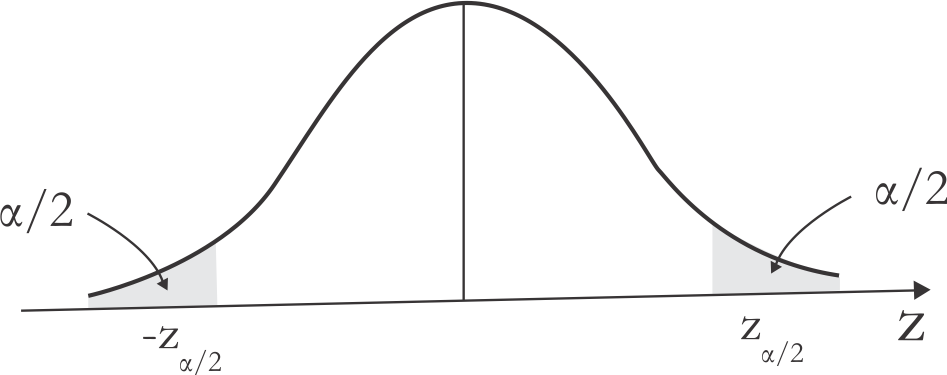
\includegraphics[width=0.6\linewidth]{fig8.8}
		\caption[]{A distribuição Z.}
	\end{figure}
	
	\begin{center}
		Desse modo, o intervalo bilateral com $95\%$ de confiança é
		\begin{equation*}
			50,52 \leq  \mu \leq52,08
		\end{equation*}
		
	\end{center}
	
	Sendo nosso intervalo de valores razoáveis, para a taxa média de queima, com $95\%$ de confiança.
	
	
	\subsection*{Escolha do tamanho da amostra}
	\vspace{0,2cm}
	\begin{blockquote}
		\begin{center}
			\vspace{0,2cm}
			\textbf{\underline {Definição}} 
		\end{center}
		
		Se $ \overline{x} $ for usada como uma estimativa de $\mu$, podemos estar $100(1-\alpha)\%$ confiantes de que o erro $|\overline{x}-1|$ não excederá um valor especificado $E$ quando o tamanho da amostra for
		
		\begin{equation*}
			n=\left(\frac{z_{\alpha / 2 }{\sigma}}{E} \right)^2
		\end{equation*}
		
		\vspace{0,2cm}
	\end{blockquote}
	\vspace{0,4cm}
	
	Note a relação geral entre o tamanho da amostra, o comprimento desejado do intervalo de confiança de $ 100 (1 - \alpha ) \% $ e o desvio-padrão $\sigma$:
	
	\begin{itemize}
		\item À medida que o comprimento desejado do intervalo $2E$ diminui, o tamanho requerido $n$ da amostra aumenta para um valor fixo de $\sigma$ e confiança especificada;
		\item  À medida que $\sigma$ aumenta, o tamanho requerido $n$ da amostra aumenta para comprimento desejado fixo $\sigma$ $2E$ e confiança especificada;
		\item À medida que o nível de confiança aumenta, o tamanho requerido $n$ da amostra aumenta para o comprimento desejado fixo $2E$ e desvio-padrão $\sigma$.
		
	\end{itemize}
	
	\newpage 
	\subsection*{Intervalo Unilateral de Confiança}
	É também possível obter intervalos unilaterais de confiança para $\mu$, estabelecendo $l=-\infty$ ou $\mu=\infty$ e trocando $z_{\alpha/2}$ por $z_{\alpha}$.
	
	
	\vspace{0,2cm}
	\begin{blockquote}
		\begin{center} 
			\textbf{O intervalo superior com $100(1-\alpha)\%$ de confiança para $ \mu $ é} 
		\end{center}
		
		
		\begin{equation*}
			\mu \leq  u = \overline{x} + z_{\alpha} 
		\end{equation*}
		\begin{center} \textbf{e o intervalo inferior com $100(1-\alpha)\%$ de confiança para $ \mu $ é}
		\end{center}
		\begin{equation*}
			\overline{x} -z_{\alpha}{\sigma} /\sqrt{n} =  l \leq \mu
		\end{equation*}
	\end{blockquote}
	\vspace{0,4cm}
	
	\subsection*{8.2.7. Método Geral para reduzir um intervalo de Confiança}
	
	É fácil dar um método geral para encontrar um intervalo de confiança para parâmetro desconhecio $\theta$. Faça $X1, X2,...X$, ser uma amostra aleatória com $n$ observações. Suponha que possamos encontrar uma estatística $g(X1, X2,...X,;\theta)$ com as seguintes propriedades:
	\begin{enumerate}
		\item $g(X1, X2, ..., Xn:\theta$) depende da amostra e de $\theta$ e
		\item{a distribuição de probabilidade de $g(X1, X2, ..., X: \theta)$ não depende de $\theta$ ou de qualquer outro parâmetro desconhecido.}
	\end{enumerate}
	
	
	No caso considerado nessa seção, o parâmetro $\theta \ = \mu$. A variável aleatória $g(X1, X2, ..., X_n:\mu)$ = $(\overline{X}-\mu)/({\sigma} /\sqrt{n})$ satisfaz ambas as condições anteriores; ela depende da amostra e de $\mu$ e tem uma distribuição normal padrão desde que $\theta$ seja conhecido. Agora, tem-se de encontrar as constantes $C_L$ e $C_U$ de modo a 
	
	\begin{equation*}
		P[C_L \leq g(X_1, X_2, ..., X_n; \theta) \leq C_U] = 1 - \alpha
	\end{equation*}
	Devido à propriedade $2, C_L$ e $C_U$ não depende de $\theta$. Em nosso exemplo, $C_L = z_{\alpha/2}$ e $C_U = z_{\alpha/2}$. Finalmente, você tem de manipular as desigualdades no enuciado de probabilidade, de modo a 
	
	\begin{equation*}
		P[L(X_1, X_2, ..., X_n) \leq \theta \leq U(X_1, X_2, ..., X_n)] = 1 - \alpha
	\end{equation*} \
	
	Isso fornece $L(X_1, X_2, ..., X_n)$ e $U(X_1, X_2, ..., X_n)$ como os limites inferiores e superiores de confiança, definindo o intervalo de confiança de $100(1-\alpha)\%$ para $\theta$. Em nosso exemplo, encontramos $L(X_1, X_2, ..., X_n)= \overline{X} -z_{\alpha}{\sigma} /\sqrt{n}$ e $U(X_1, X_2, ..., X_n)= \overline{X} +z_{\alpha}{\sigma} /\sqrt{n}$.
	
	\newpage
	\section*{8.3 INFERÊNCIA SOBRE A MÉDIA DE UMA POPULAÇÃO COM VARIÂNCIA DESCONHECIDA}
	
	Quando estamos testando hipóteses ou construíndo intervalos de confiaça para a média $\mu$ de uma população quando $\sigma^2$ for deseconhecida, podemos usar os procedimentos de testes da Seção 8.2. Entretanto, quando a amostra for pequena e $\sigma^2$ for desconhecida, teremos de fazer uma suposição sobre a forma de distribuição em estudo de modo a obter um procedimento de teste. Uma suposição razoável, em muitos casos, é que a distribuição sob consideração seja normal.
	
	\subsection*{8.3.1 Testes de Hipóteses para a Média}
	
	Suponha que a população de interesse tenha distribuição normal, com a média $\mu$ e variância $\sigma^2$ desconhecidas. Desejamos testar a hipótese de que $\mu$ seja igual a uma constante $\mu_o$. Note que essa situação é similar àquela da Seção 8.2, exeto que agora ambas, $\mu$ e $\sigma^2$, são desconhecidas. Considere que uma da amostra aleatória de tamanho $n$, como $X1, X2, ... Xn$. seja disponível e sejam $\overline{X}$ e $S^2$ a média e a variância amostral, respectivamente. 
	Desejamos testar a hipótese alternativa bilateral.
	
	\newpage
	
	\begin{center} % Everything within the center environment is centered.
		{\Large \bf Trabalho1 - Latex - Escrita do arquivo Trabalho4-LAtex.pdf} % <---- Don't forget to put in the right number
		\vspace{2mm}
		
	\end{center}  

	\vspace{0.4cm}
	
	\begin{align*}
			H_0: \mu = \mu_0 \\
			H_1: \mu \pm \mu_0
	\end{align*}

	Se a variância $\sigma^2$ for conhecida, a estatística de teste será a Eq. 8.10:
	
	\begin{equation*}
		Z_0 = \frac{\overline{X} - \mu_0}{\sigma / \sqrt{n}}
	\end{equation*}

	Quando $\sigma^2$ for desconhecida, um procedimento lógico será trocar $\sigma$ na Eq. 9.10 pelo desvio-padrão, S, da amostra. A estatística de teste é agora
	
	\begin{blockquote}
		\begin{equation}
			\tag{8.39}
			T_0 = \frac{\overline{X} - \mu_0}{S / \sqrt{n}}
		\end{equation}  
	\end{blockquote}
	
	Uma questão lógica é qual o efeito de trocar $\sigma$ por $S$ na distribuição da estatística $T_0$? Se $n$ for grande, a resposta a essa questão é "muito pouco" e podemos usar o procedimento de teste baseado na distribuição normal da seção 8.2. Entretanto, n é geralmente pequeno na maioria dos problemas de engenharia e nessa situação uma distribuição diferente tem de ser empregada.
	
	\begin{blockquote}
		\begin{center}
			\textbf{\underline{Definição} } 
		\end{center}
		
		Faça $ X_1 $, $ X_2 $, ... , $ X_n $ ser uma amostra aleatória para uma distribuição normal, com média $\mu$  e variância $\sigma^2$ desconhecida. A grandeza
		
		\begin{equation*}
			T = \frac{\overline{X} - \mu_0}{S / \sqrt{n}}
		\end{equation*}
		
		
		tem uma distribuição $ t $, com $ n-1 $ graus de liberdade.
	\end{blockquote}

	A função densidade da probabilidade $t$ é
	\begin{equation*}
		\tag{8.40}
		f(x) = \frac{\Gamma \left[ \left( k + 1 \right) /2 \right] }{\sqrt{ \pi k  }\Gamma \left( k/2 \right)  } . \frac{1}{\left[ \left( x^2 / k \right) + 1  \right]^{\left( k+1 \right)/2 } } - \infty  < x < \infty 
	\end{equation*}

	sendo $k$ o número de graus de liberdade. A média e a variância da distribuição $t$ são iguais a zero e $ k/(k-2) $(para $  k > 2 $), respectivamente.
	
	\hspace{12pt} Várias distribuições $t$ são mostradas na Figura \ref{8.11}.
	
	
	\begin{figure}[H]
		\centering
		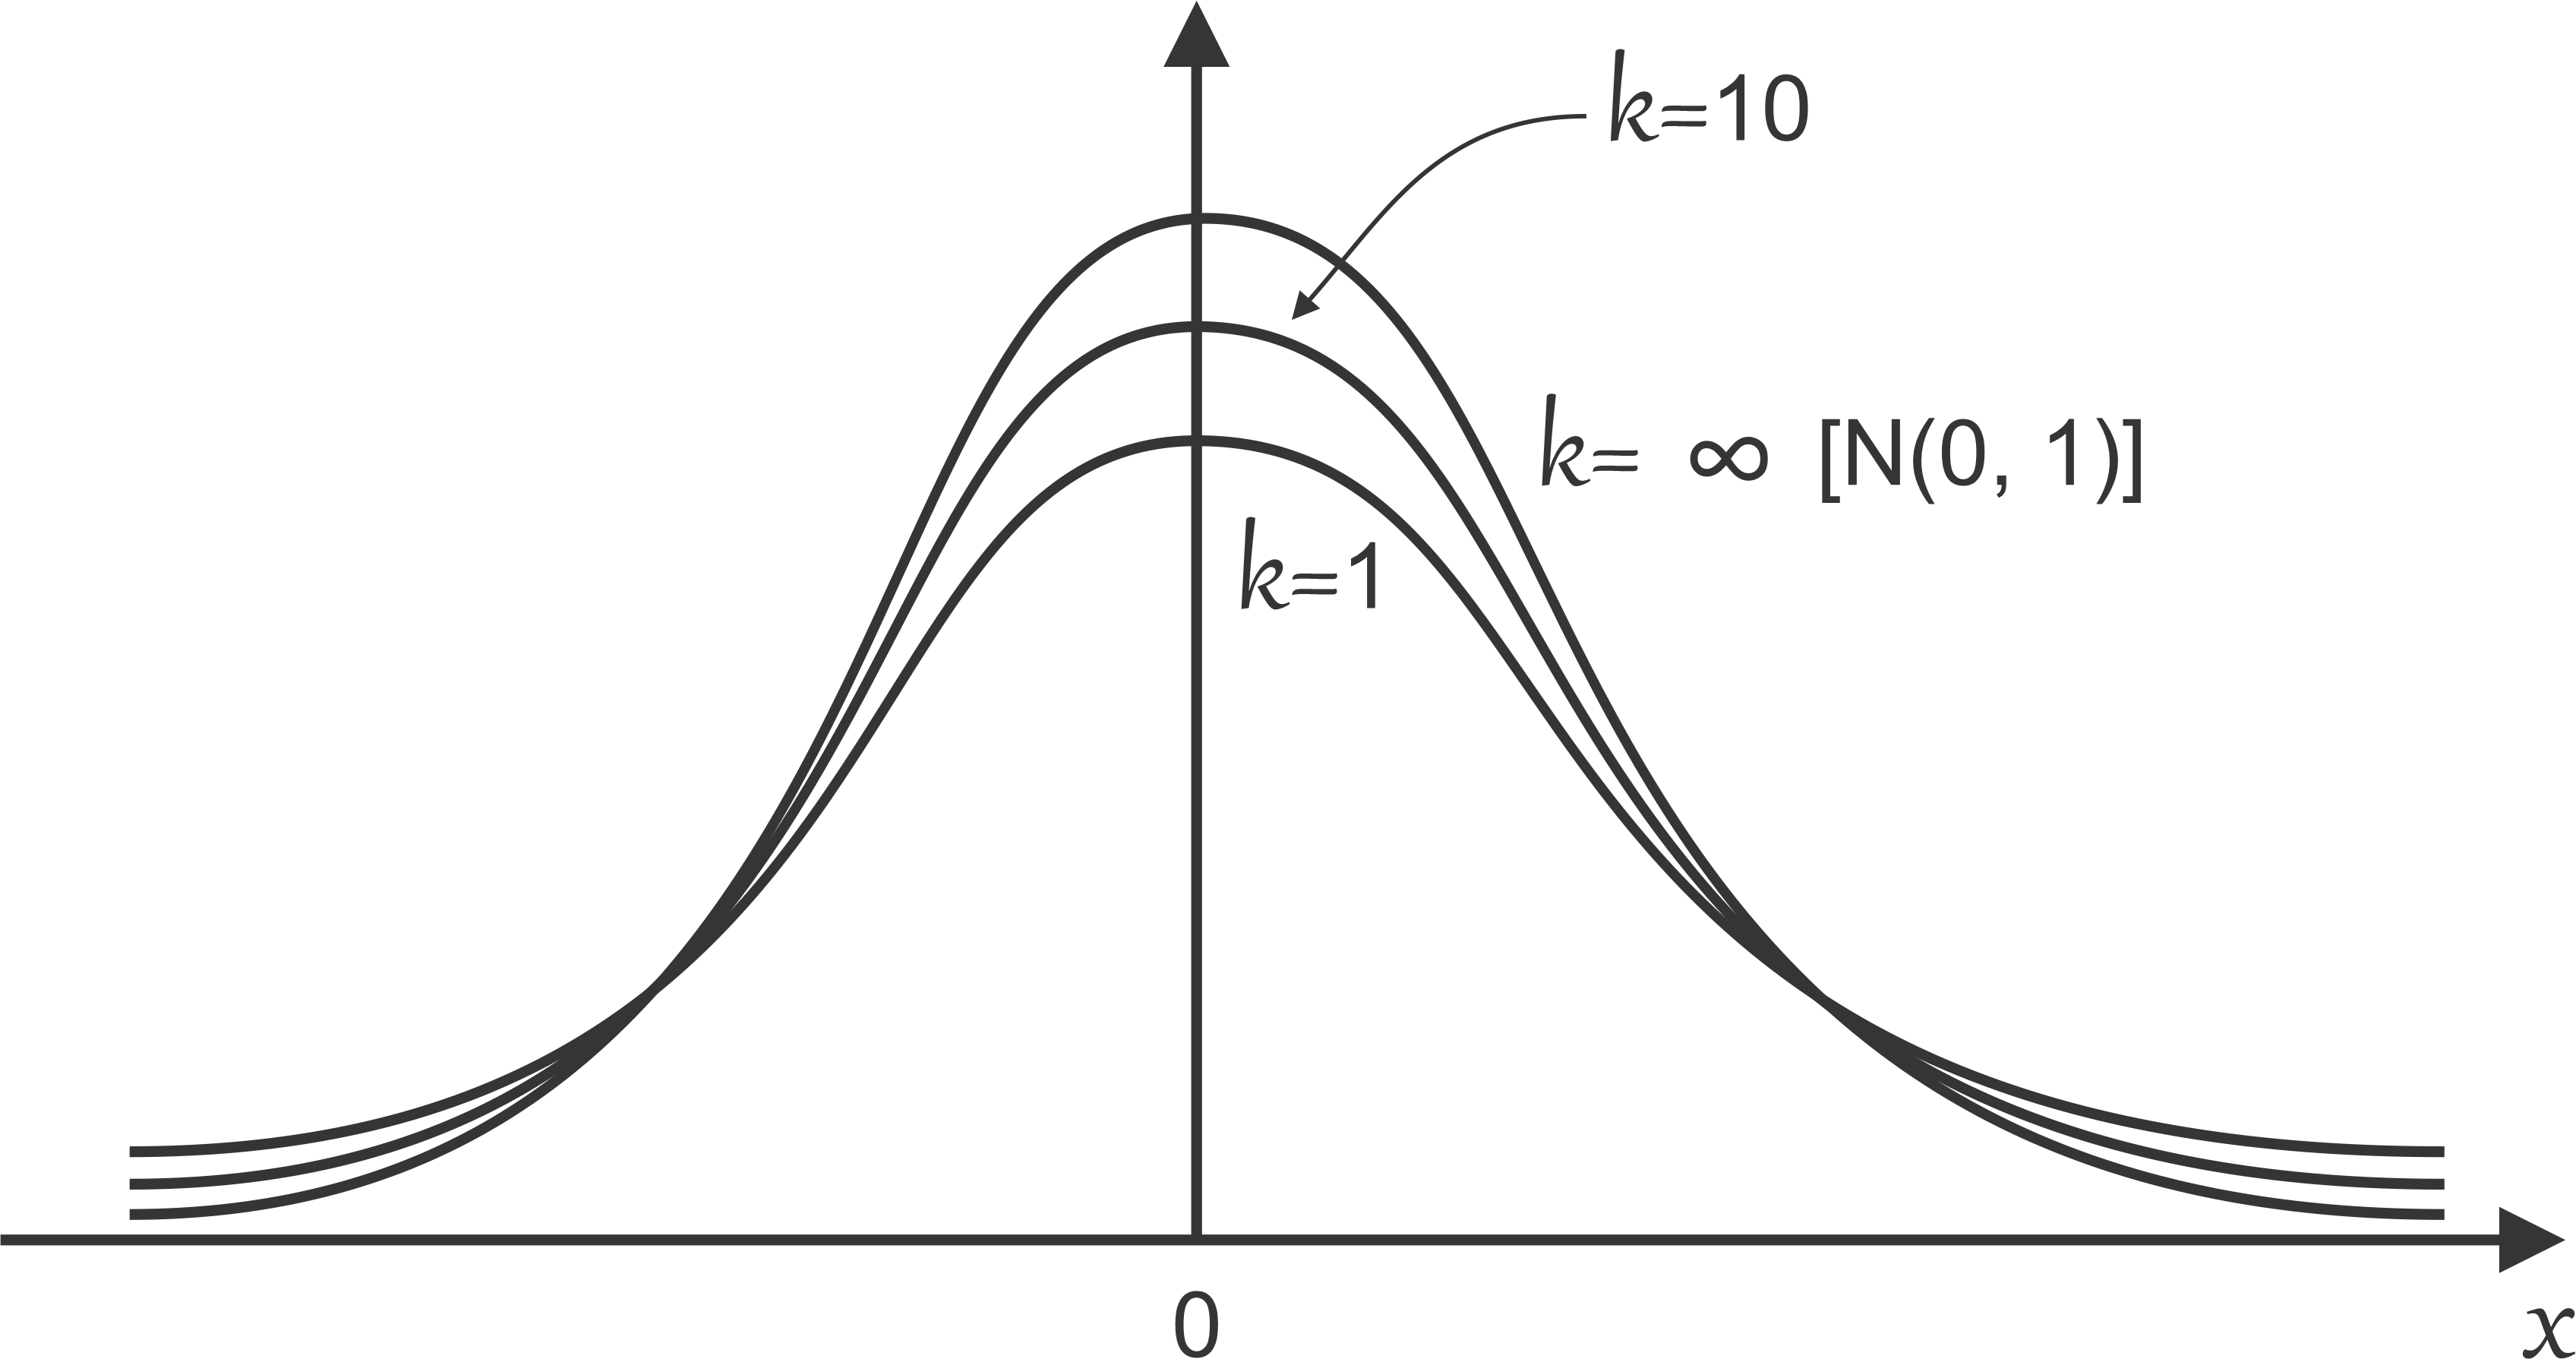
\includegraphics[width=0.7\linewidth]{fig1}
		\caption[]{Funções densidade de probabilidade de várias distribuições t.}
		\label{8.11}
	\end{figure}

	Agora, pode-se ver, de forma direta, que a distribuição da estatística de teste na Eq.8.39 é $t$, com $n-1$ graus de liberdade, se a hipótese nula $H_0: \mu = \mu_0$ for verdadeira. Para testar $H_0: \mu = \mu_0$, o valor da estatística de teste $t_0$ na Eq.8.39 é calculado e $H_0$ é rejeitada se
	\begin{equation}
		\tag{8.41a}
		t_0 > t_{\alpha / 2, n-1}
	\end{equation}
	ou
	\begin{equation}
		\tag{8.41b}
		t_0 < - t_{\alpha / 2, n-1}
	\end{equation}

	em que $t_0 > t_{\alpha / 2, n-1}$ e $t_0 < - t_{\alpha / 2, n-1}$ são pontos $100 \alpha / 2 \%$ superior e inferior da distribuição $t$, com $n-1$ graus de liberdade, definidos previamente.
	
	\hspace*{12pt} Para a hipótese alternativa unilateral
	\begin{equation*}
		H_0: \mu = \mu_0
	\end{equation*}
	
	\begin{equation}
		\tag{8.42}
		H_1: \mu > \mu_0
	\end{equation}
	Calculamos a estatística de teste $t_0$, a partir da Eq. 8.9, e rejeitamos %H_0% se
	\begin{equation}
		\tag{8.43}
		t_0 >  t_{\alpha, n-1}
	\end{equation}

	Para a outra hipótese alternativa unilateral
	\begin{equation*}
		H_0: \mu = \mu_0
	\end{equation*}
	\begin{equation}
		\tag{8.44}
		H_1: \mu < \mu_0
	\end{equation}

	\begin{figure}[H]
		\centering
		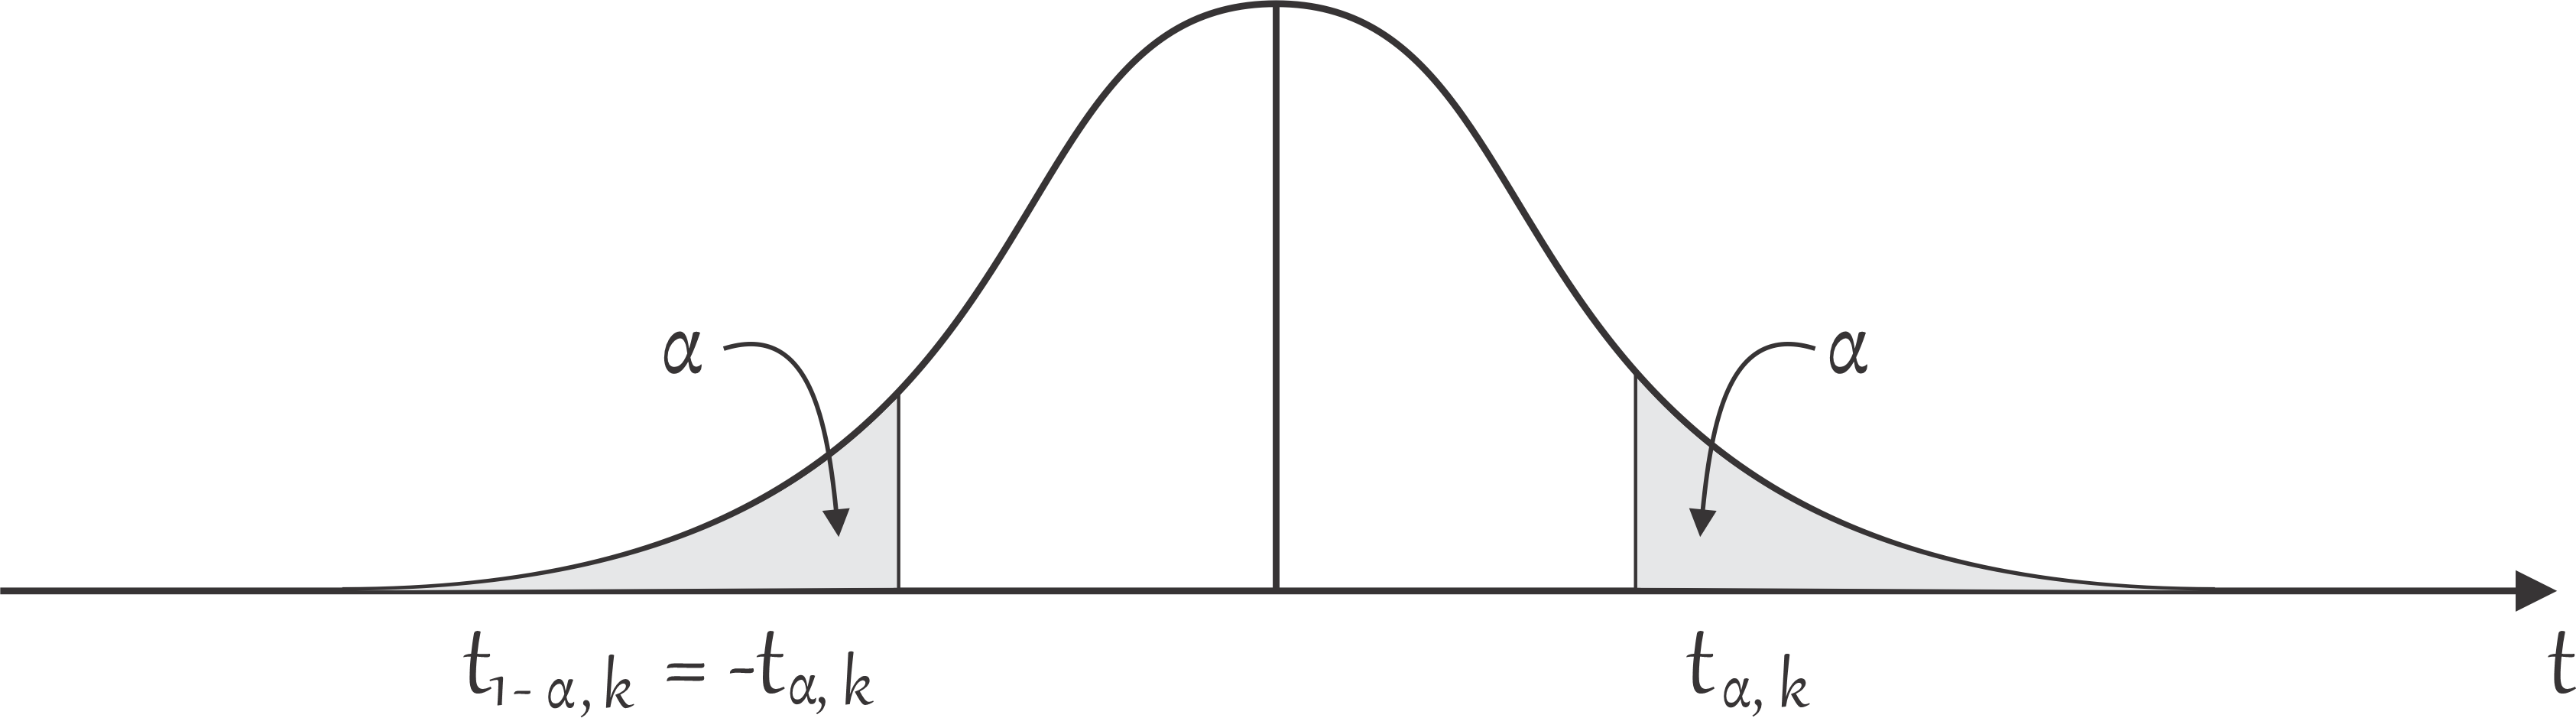
\includegraphics[width=0.7\linewidth]{fig2}
		\caption[]{pontos percentuais da distribuições t.}
	
	\end{figure}

	rejeitamos $H_0$ se
	\begin{equation}
		\tag{8.45}
		t_0 < -t_{\alpha, n-1}
	\end{equation}

	\section*{EXEMPLO 8.8}
	Um artigo no periódico Materials Engineering (1989, Vol.II, No. 4, pp. 275-281) descreve os resultados de testes de tensão quanto à adesão em 22 corpos de prova de liga U-700. A carga no ponto de falha do corpo de prova é dada a seguir (em MPa):
	\begin{table}[H]
		\centering
		\begin{tabular}{lllll}
			\hline
			19,8 & 18,5 & 17,6 & 16,7 & 15,8 \\
			15,4 & 14,1 & 13,6 & 11,9 & 11,4 \\
			11,4 & 8,8  & 7,5  & 15,4 & 15,4 \\
			19,5 & 14,9 & 12,7 & 11,9 & 11,4 \\
			10,1 & 7,9  &      &      &      \\ 
			
			\hline
		\end{tabular}
	\end{table}

	A média amostral é $ \overline{x} = 13,71  $ e o desvio-padrão é $s=3,55$. Os dados sugerem que a carga média na falha excede 10MPa? Considere que a carga na falha tenha uma distribuição normal e use $ \alpha = 0,05 $.
	
	\hspace{10pt} A solução, usando o procedimento de 8 etapas para o teste de hipóteses, é dada a seguir:
	\begin{enumerate}
		\item O parâmetro de interesse é a carga média na falha, $\mu$.
		\item $H_0$:$\mu = 10$
		\item $H_1$:$\mu > 10$. Queremos rejeitar $H_0$ se a carga média na falha exceder 10MPa.
		\item $\alpha = 0,05$.
		\item A estatística de teste é
		\begin{equation*}
			t_0 = \frac{\overline{x} - \mu_0}{s/ \sqrt{n}}
		\end{equation*}
		\item Rejeite $H_0$ se $t_0 > t_{0,05, 21} = 3,55$, $\mu = 10$ e $n=22$, temos 
		\begin{equation*}
			t_0 = \frac{13,71 - 10}{3,55 / \sqrt{22}} = 4,90
		\end{equation*}
	
		\item Conclusões: Uma vez que $ t_0 = 4,90 > 1,721 $, rejeitamos $H_0$ e concluímos, com um nível de 0,05 de significância, que a carga média da falha excede 10 MPa. 
	\end{enumerate}

	\section*{8.3.5 Intervalo de Confiança para a Média}
	É fácil encontrar um intervalo de confiança de $100(1- \alpha)\%$ para a média de uma distribuição normal com variância desconhecida, procedendo como fizemos na Seção 8.2.6. Em geral, a distribuição de $T= \left( \overline{X} - \mu \right) / \left( S/ \sqrt{n} \right)  $ é $t$, com $n-1$ graus de liberdade. Fazendo $t_{\alpha / 2, n-1}$ ser o ponto superior $100 \alpha / 2 \%$ da dsitribuição t, com n-1 graus de liberdade, podemos escrever:
	\begin{equation*}
		P\left( -t_{\alpha / 2, n-1} \leq T \leq t_{\alpha / 2, n-1} \right) 
	\end{equation*}
	ou
	\begin{equation*}
		P\left( -t_{\alpha / 2, n-1} \leq  \frac{\overline{X} - \mu_0}{S/ \sqrt{n}} \leq t_{\alpha / 2, n-1} \right) 
	\end{equation*}

	Rearranjando essa última equação, resulta em
	
	\begin{equation*}
		\tag{8.49}
		P\left(\overline{X} -t_{\alpha / 2, n-1}S/ \sqrt{n} \leq  \mu \leq \overline{X} + t_{\alpha / 2, n-1}S/ \sqrt{n} \right) = 1- \alpha
	\end{equation*}

	Isso conduz á seguinte definição de intervalo bilateral de confiança com  $100 \left(1- \alpha \right)  \%$ para $ \mu $.
	
	\begin{blockquote}
		\begin{center}
			\textbf{Definição: Intervalo de Confiança para Média de uma} \textbf{\underline{Distribuição Normal com Variância Desconhecida}}  
		\end{center}
		
		Se $\overline{x}$ e $s$ forem a média e o desvio-padrão de uma amostra aleatória proveniente de uma população normal, com variância desconhecida $\sigma^2$, então um intervalo de confiança de $100 \left(1- \alpha \right)  \%$ para a média $\mu$ é dado por
		
		\begin{equation*}
			\tag{8.50}
			\overline{x} -t_{\alpha / 2, n-1}S/ \sqrt{n} \leq  \mu \leq \overline{x} + t_{\alpha / 2, n-1}S/ \sqrt{n}
		\end{equation*}
		sendo $ t_{\alpha / 2, n-1} $ o ponto superior $100 \alpha / 2 \%$ da distribuição $t$, com $n-1$ graus de liberdade.
	\end{blockquote}

	Intervalos unilaterais de confiança para a média de uma distribuição normal são também de interesse e são fáceis de usar. Use simplesmente somente o limite inferior ou superior apropriado de (8.50) e troque $ t_{\alpha / 2, n-1} $ por $ t_{\alpha, n-1} $.
	
	
	\section*{EXEMPLO 8.10}
	Reconsidere o problema da tensão quanto à adesão no Exemplo 8.8. Sabemos que $n = 22$, $\overline{x} = 13,71$, $s=3,55$. Encontraremos um intervalo de confiança de $ 95\% $ para $\mu$. Da Eq. 8.50, encontramos $ \left(t_{\alpha / 2, n-1} = t_{0,025; 21} = 2,080 \right)  $:
	\begin{align*} 
		\overline{x} - t_{\alpha / 2, n-1} s \sqrt{n}  & \leq \mu \leq  \overline{x} + t_{\alpha / 2, n-1} s \sqrt{n}  \\ 
		13,71 - 2,080 \left( 3,55 \right) / \sqrt{22}  & \leq \mu \leq  13,71 + 2,080 \left( 3,55 \right) / \sqrt{22}  \\
		13,71 - 1,57  & \leq \mu \leq  13,71 + 1,57 \\
		12,14  & \leq \mu \leq  15,28
	\end{align*}
	No exemplo 8.8, testamos uma hipótese alternativa unilateral para $ \mu $. Alguns engenheiros podem estar interessados em um intervalo inferior de confiança de $95\%$ para a carga média na falha é encontrado usando o limite inferior de confiança de (8.50), com $t_{\alpha / 2, n-1}$ trocado por $t_{\alpha, n-1}$, isso conduz a:
	\begin{align*} 
		\overline{X} - t_{0,05, n-1} S \sqrt{n}  & \leq \mu  \\ 
		13,71 - 1,721 \left( 3,25 \right) / \sqrt{22}  & \leq \mu  \\ 
		12,52 & \leq \mu
	\end{align*}

	Logo, podemos dizer com $95\%$ de confiança que a carga média na falha excede 12,52 MPa.
	
	

	
	
	
\end{document}
	